\chapter{Background}
\label{sec:background}

This chapter explains the most important concepts needed to understand the
algorithms that are proposed in this thesis. The first section describes
\emph{Markov decision processes (MDPs)}, the problem formalization we will use
for games. The next section describes MCTS, a tree search algorithm that is
commonly used on games and other MDPs. Subsequently, options will be formalized,
these simulate the idea of defining subgoals and how to reach them. Then, the
basics of Q-learning are described, after which SMDP Q-learning is explained.
Finally the \emph{video game description language (VGDL)} is explained. This is
the protocol that is used by the GVGAI competition to implement the many
different games the competition offers, each of which uses the same interaction
framework with the game playing algorithms.

In this thesis, games are considered to be an unknown environment and an agent
has to learn by interacting with it. After interaction, agents receive
rewards that can be either positive or negative. This type of problem is called
reinforcement learning \cite{wiering2012reinforcement}.

\section{Markov Decision Processes}
\label{subsec:mdps}
In this thesis, games will be treated as MDPs, which provide a mathematical
framework for use in decision making problems. An MDP is formally defined as a
tuple $\langle S, A, T, R \rangle$, where $S$ denotes the set of states. Since an MDP
is fully observable, a state contains all the information of the
game's current condition: locations of sprites like monsters and portals; the
location, direction and speed of the avatar; which resources the avatar has
picked up; etcetera. $A$ is a finite set of actions, the input an agent can
deliver to the game. $T$ is a transition function defined as $T : S \times A
\times S \rightarrow \left[0,1\right]$. It specifies the probabilities over the
possible next states, when taking an action in a state.  $R$ is a reward
function defined as $R: S \times A \times S \rightarrow \mathbb{R}$. In this
case, when the game score changes, the difference is viewed as the reward.
Algorithms typically maximize the cumulative reward, which is analogous to the
score. An MDP by definition has the \emph{Markov property}, which means that the
conditional probability distribution of future states depends only upon the
present state. No information from previous states is needed. Algorithms do not
have access to $T$ and $R$ in the scope of this thesis.

For example, for the game Zelda, a state $s$ consists of the location, rotation
and speed of the avatar and the location of the avatar's sword, the monsters, the
walls and the key and portal that need to be found. $S$ is the set of all
possible states, so all possible combinations of these variables. The action set
$A$ consists of the movement actions \textsc{up}, \textsc{down}, \textsc{left}
and \textsc{right}, and \textsc{use}, which in this case spawns the sword in
front of the avatar for a couple of time steps. The transition function $T$
defines the transition from a state, given an action.  This means that the
transition defines the change in location of the monsters and the avatar and if
any of the sprites disappear, e.g., when the avatar picks up the key. Note that,
since the transition function is not by definition deterministic, the resulting
state from an action $a$ in state $s$ is not necessarily the same state
(a \emph{non player character} (NPC) that moves about randomly can move in any direction between
states independent of the agent's action). The reward function describes the
change in game score, given a state, action and resulting next state. For
example, when the avatar kills a monster with the action \textsc{use}, its score
will increase with 1.

An important trade-off in decision theory is the choice between exploration and
exploitation. Exploration means to use the actions that have been used little
and find out whether they lead to a reward. On the other hand, exploitation
means to use the actions that you already know will lead to a reward. When an
algorithm prioritizes exploitation over exploration too much, it has the risk of
never finding unknown states which have higher rewards. It will keep exploiting
the states with a lower reward that it has already found. In contrast, too much
exploration might lead to lower rewards, because the algorithm takes the action
that maximizes reward less often.

\section{Monte Carlo Tree Search}
\label{subsec:mcts}
Monte Carlo methods have their roots in statistical physics, where they have
been used to approximate intractable integrals. Abrahamson
\cite{abramson1990expected} demonstrated theoretically that this sampling method
might be useful for action selection in games as well.  In 2001, Monte Carlo
methods were effectively used for bridge \cite{ginsberg2001gib}. The real
success of MCTS started in 2006, when the tree search method and UCT formula
were introduced, yielding very good results in Computer Go
\cite{gelly2006modification}. Since 2006, the algorithm has been extended with
many variations and is still being used for other (computer) games
\cite{browne2012survey}, including the GVGAI competition
\cite{perez2014knowledge}.

\begin{figure}
	\centering
	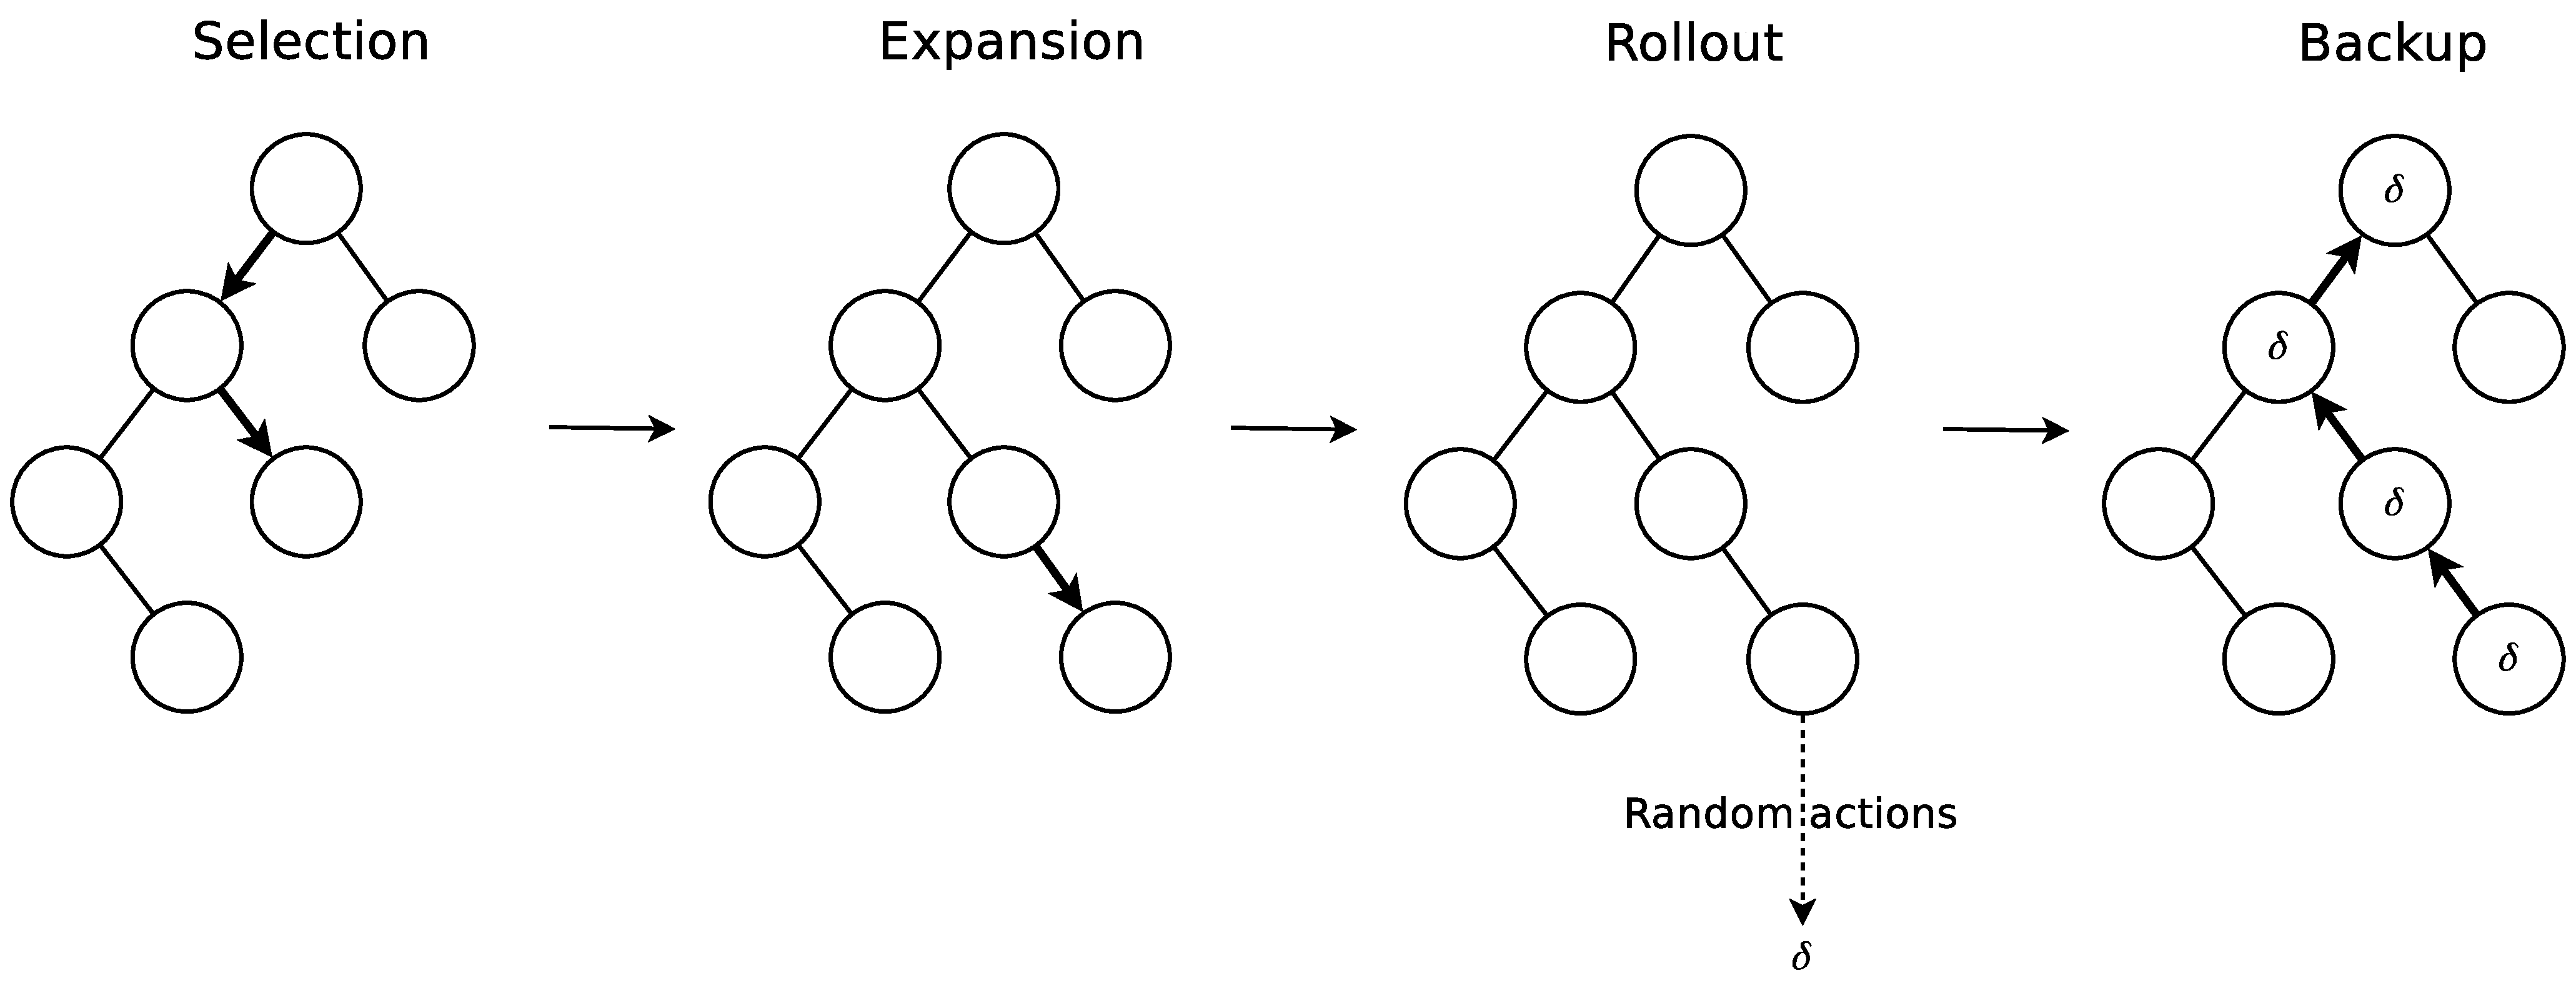
\epsfig{file=includes/mcts-wide.eps, width=\textwidth}
	\caption{One Monte Carlo tree search iteration}
	\label{fig:mcts}
\end{figure}

This section explains how MCTS approximates action values for states.  A tree is
built incrementally from the states and actions that are visited in a game. Each
node in the tree represents a state and each connection in the tree represents
an action taken in that state leading to a new state, which is represented by
the next tree node.  The process, as explained in Figure \ref{fig:mcts},
consists of four phases that are constantly repeated. It is started with the
current game state, which is represented by the root node of the tree. The first
action is chosen by an \emph{expansion} strategy and subsequently simulated.
This results in a new game state, for which a new node is created. After
expansion, a \emph{rollout} is done from the new node, which means that a
simulation is run from the new node applying random actions until a predefined
stop criterion is met or the game ends. Finally, the score difference resulting
from the rollout is \emph{backed up} to the root node, which means that the
reward is saved to the visited nodes.  Then a new iteration starts. When all
actions are expanded in a node, that node is deemed \emph{fully expanded}.
This means that MCTS will use its \emph{selection} strategy to select child
nodes until a node is selected that is not fully expanded.  Then, the expansion
strategy is used to create a new node, after which a rollout takes place and the
results are backed up.

The selection strategy selects optimal actions in internal tree nodes by
analyzing the values of their child nodes. An effective and popular
selection strategy is the \emph{upper confidence tree (UCT)}
\cite{kocsis2006bandit}. This balances the choice between poorly explored
actions with a high uncertainty about their value and actions that have been
explored extensively, but have a higher value. A child node $j$ is selected to
maximize
\begin{equation}
	\label{eq:uct}
	UCT = v_{s'} C_p \sqrt{\frac{2 \ln n_s}{n_{s'}}}
\end{equation}
Where $v_{s'}$ is the value of child $s'$ as calculated by the backup function,
$n_s$ is the number of times the current node $s$ has been visited, $n_{s'}$ is
the number of times child $s'$ has been visited and $C_p > 0$ is a constant
that shifts priority from exploration to exploitation. By increasing $C_p$, the
priority is shifted to exploration: states that have been visited less, will be
visited with a higher priority than states that have been visited more. A
decrease shifts priority to exploitation: states that have a high value are
visited more, in order to maximize reward. 

The traditional expansion strategy is to explore each action at least once in
each node. After all actions have been expanded, the node applies the selection
strategy for further exploration. Some variants of MCTS reduce the branching
factor of the tree by only expanding the nodes selected by a special expansion
strategy. A specific example is the \emph{crazy stone} algorithm
\cite{coulom2007efficient}, which is an expansion strategy that was designed
specifically for Go. We will use an adaptation of this strategy in the algorithm
proposed in Chapter \ref{sec:learning}.  When using crazy stone, an action $i$
is selected with a probability proportional to $u_i$
\begin{equation}
	\label{eq:crazystone}
	u_i = \exp\left(K \frac{\mu_0 - \mu_i}{\sqrt{2\left(\sigma_0^2 +
\sigma_i^2\right)}}\right) + \varepsilon_i
\end{equation}
Each action has an estimated value $\mu_i$ ordered in such a way that $\mu_0 >
\mu_1 > \ldots > \mu_N$, and a variance $\sigma_i^2$. K is a constant
that influences the exploration -- exploitation trade off. $\varepsilon_i$ prevents
the probability of selecting a move to reach zero and its value is proportional
to the ordering of the expected values of the possible actions. 
\begin{equation}
	\label{eq:epsilon}
	\varepsilon_i = \frac{0.1 + 2^{-i} + a_i}{N}
\end{equation}
Where $a_i$ is 1 when an action is \emph{an atari move}, a go-specific
move that can otherwise easily be underestimated by MCTS, and otherwise 0.

After a rollout, the reward is backed up, which means that the estimated value
for every node that has been visited in this iteration is updated with the
reward of this simulation. Usually the estimated value of a node is the average
of all rewards backed up to that node.


\section{Options}
\label{subsec:options}

In order to mimic human game playing strategies, such as defining subgoals and
subtasks, we use options. Options have been proposed by Sutton et al.  as a
method to incorporate temporal abstraction in the field of reinforcement
learning \cite{sutton1999between}. The majority of the research seems to focus
on learning algorithms and little work has been done on combining options with
tree search methods, which offer a model free planning framework
\cite{barto2003recent}.

An option, sometimes referred to as a macro-action, is a predefined method of
reaching a specific subgoal. Formally, it is a triple $\langle I, \pi, \beta
\rangle$ in which $I \subseteq S$ is an initiation set, $\pi: S \times A
\rightarrow [0, 1]$ is a policy and $\beta: S^+ \rightarrow [0,1]$ is a
termination condition. The initiation set $I$ is a set of states in which the
option can be started. This set can be different for each option. The option's
policy $\pi$ defines the actions that should be taken for each state. The
termination condition $\beta$ is used to decide if an option is finished, given
that the agent arrived at a certain state.

When an agent starts in state $s$, it can choose from all of the options $o \in
O$ that have $s$ in its initiation set $I_o$. Then the option's policy $\pi$ is
followed, possibly for several time steps. The agent stops following the policy
as soon as it reaches a state that satisfies a termination condition in $\beta$.
This often means that the option has reached its subgoal, or a criterion is met
that renders the option obsolete (e.g., its goal does not exist anymore).
Afterwards, the agent chooses a new option that will be followed.

Using options in an MDP removes the Markov property for that process: the state
information alone is no longer enough to predict an agent's actions, since the
actions are now not only state-dependant, but dependant on what option the agent
has chosen in the past as well. According to \cite{sutton1999between}, we can
view the process as a \emph{semi-Markov decision process (SMDP)}
\cite{duff1995reinforcement}, in which options are actions of variable length.
In this thesis, we will call the original action set of the MDP $A$, and the set
of options $O$.

Normally, an agent can never choose a new option in a state that is not in the
termination set of any of the options. Some algorithms use \emph{interruption},
which means they are designed not to follow an option until its stop criterion
is met, but choose a new option every time step \cite{sutton1999between,
precup2000temporal}. Using this method, an agent can choose a new option in any
state that is present in the MDP, which can lead to better performance than
without interruption.

Most options span over several actions. Their rewards are discounted over time.
This means that rewards that lay further in the future are valued less than
those that lay nearer. A reward $r_o$ for option $o$ is calculated for using an
option from timestep $t$ to timestep $t+n$ with
\begin{equation}
	\label{eq:option-reward}
	r_o = r_{t} + \gamma r_{t+1} + \gamma^2 r_{t+2} + \cdots + \gamma^n r_{t+n},
\end{equation}
where $\gamma$ is the discount factor, which indicates the importance of future
states. 

Normal actions can be treated as options as
well.  An option for action $a \in A$ has a initiation set $I = S$, the policy
$\pi$ is taking action $a$ in all the states.  The termination condition $\beta$
is that action $a$ should be performed once. 

\section{Q-learning}
\label{subsec:qlearning}
Q-learning is a relatively simple method for reinforcement learning,
that was proposed in 1992 \cite{watkins1992q}. The \emph{Q-value} of an action
for a state, $Q(s, a)$, is the discounted reward that can be achieved by
applying action $a$ to state $s$ and following the optimal policy afterwards. By
learning Q-values for every action in every state, it can estimate an optimal
policy. 

The general idea of Q-learning is to incrementally save the combination of a
reward and the current estimate of the Q-value of an action and game state.
An agent starts in state $s$, takes action $a$ and arrives in state $s'$ with
reward $r$.  The update function uses the reward and the maximum of the Q-values of the
next state $s'$. By always using the maximum value of the next state, the Q-value
function will eventually converge the maximum discounted future reward for a
state-action pair. The update function for a state-action pair is denoted by 
\begin{equation}
	\label{eq:qlearning}
	Q(s, a) \gets Q(s, a) + \alpha \left(r + \gamma \max_{a' \in A} Q(s', a') - Q(s, a)\right),
\end{equation}
where $r$ is the reward that is achieved by using action $a$ in state $s$,
leading to state $s'$. The algorithm has two parameters: $\gamma$ is the
discount factor and $\alpha$ is the learning rate, which determines the
magnitude of the Q-value updates.  Q-learning is shown to converge if $\alpha$
decreases over time. However, in practice it is often set to a small constant.
The Q-table can be used to find the optimal policy by, for each state $s \in S$,
selecting the action $a \in A$ that maximizes $Q(s, a)$. Because after each action
only one state-action pair is being updated, Q-learning can take a long time to
converge. It is, however, guaranteed to converge to the optimal policy, given that
during exploration each state-action pair is visited an infinite number of times.

\section{SMDP Q-learning}
\label{subsec:smdp-qlearning}
When options were introduced, they were used in combination with Q-learning. In
order to be able to compare our contribution to the Q-learning approach, we
implement \emph{SMDP Q-learning} \cite{sutton1999between} for VGDL, based on the
description made by Sutton et al. in section 3.2 of their paper. In general,
SMDP Q-learning estimates the expected rewards for using an option in a certain
state, in order to find an optimal policy over the option set $O$.

Like traditional Q-learning, SMDP Q-learning estimates a value function. The
option-value function contains the expected return $Q(s, o)$ of using an option
$o \in O$ in state $s \in S$. Updates of the $Q$ function are done after each
option termination by an adaptation of the original Q-learning update function
from Equation \ref{eq:qlearning}:
\begin{equation}
	\label{eq:smdp-qlearning}
	Q(s, o) \gets Q(s, o) + \alpha \left(r + \gamma^k \max_{o' \in O_{s'}}Q(s',
	o') - Q(s, o)\right),
\end{equation}
where $\gamma$ is the discount factor, $k$ denotes the number of time steps
between the start state $s$ and stop state $s'$ for option $o$, $r$ denotes
the cumulative and discounted option reward from Equation
\ref{eq:option-reward}, and step size parameter $\alpha$ is similar to the
learning rate parameter from traditional Q-learning.  The difference with
Equation \ref{eq:qlearning} is that here we take the $k$\textsuperscript{th}
power of $\gamma$, which penalizes options that take more actions. Hereby, the
desired effect is reached that an option that takes half the time, but has more
than double the reward of another option gets preferred over the other.

Using the Q-table, an option policy can be constructed. A \emph{greedy policy}
selects the option that maximizes the expected return $Q(s, o)$ for any state
$s \in S$ and option $o \in O$ with $s$ in its initiation set $I_o$. When a Q-table
is fully converged, the greedy policy is the optimal policy\footnote{Note that
it is optimal for the maximum achievable by using only the options in the option
set $O$.} \cite{sutton1999between}. Exploration is often done by using an
\emph{$\varepsilon$-greedy policy}. This is a policy that chooses a random option
with probability $\varepsilon$ and the greedy option otherwise. The parameter
$\varepsilon$ is set to a value between 0 and 1. A higher value for $\varepsilon$
leads more exploration of unknown states, whereas a lower value shifts the
algorithm's focus to exploiting the currently known feasible states.

\section{Generalized Video Game Playing}
\label{subsec:vgdl}

In this thesis, algorithms will be benchmarked on the general video game playing
problem. Recent developments in this area include the \emph{video game
description language (VGDL)} \cite{schaul2013video}, a framework in which a
large number of games can be defined and accessed in a similar manner.
VGDL aims to be a clear, human readable and unambiguous description language for
games. Games are easy to parse and it is possible to automatically generate
them. Using a VGDL framework, algorithms can access all the games in a similar
manner, resulting in a method to compare their performances on several games.

To define a game in VGDL, two files are required. Firstly, the game description
should be made, which defines for each type of object what character in the
level description it corresponds to, what it looks like in a game visualization,
how it interacts with the rest of the game and when it disappears from the
game. Secondly, a level description file is needed, in which each character maps
to an object in the game. The location in the file corresponds to its grid
location in the game. By defining these two files, a wide spectrum of games
can be created. A more extensive explanation and an example of a game in VGDL
can be found in Section \ref{subsec:games}.

The General Video Game AI competition provides games written in VGDL.
Furthermore, it provides a Java framework in which algorithms can be
benchmarked using a static set of rules. Algorithms are only allowed to observe
the game information: score, game tick (timestep), the set of possible actions
and information about if the game is over and if the player won; avatar
information: its position, orientation, speed and resources; and screen
information: Which sprites are on the screen, including their location and the
size (in pixels) of the level grid's blocks.

Algorithms have a limited amount of time to plan their actions, during which
they can access a simulator called the \emph{forward model}. The forward model
acts as a black box that returns a new state when an algorithm applies an
action. The actions that are used on the forward model do not influence the real
game score. Before the simulation time runs out, the algorithm should return an
action to apply to the real game.

The algorithms proposed in this thesis will be benchmarked on the GVGAI game
sets, using the rules of the competition. This means that the algorithms do not
have any access to the game and level descriptions. When an algorithms starts
playing a game, it typically knows nothing of the game, except for the
observations described above.
